% 原印刷235--248页／PDF物理259--272；§6.4，包含两小节，至章末.
\subsection{讨论}\label{sec:6.4}
\subsubsection{离散数值方法}\label{sec:6.4.1}
在\autoref{sec:1}中，我们大量利用了Kantorovich问题的线性与凸结构；它实际上是一个无限维线性规划问题. 因而很自然地希望寻找在离散化后利用这一事实的方法. 这里，离散化只是把$\mu$和$\nu$替换为两个有限原子测度$\mu=\sum_{i=1}^N a_i\delta_{x_i}$和$\nu=\sum_{j=1}^M b_j\delta_{y_j}$. 对固定的$N$与$M$，如何选择“最优”的点$x_i,y_j$及权重$a_i,b_j$，使逼近尽可能精确，是我们不打算在此讨论的微妙问题. \phantomsection\label{idx:i124-p236}\index{Q124@量化（quantization）|hyperpage}
它与测度$\mu,\nu$的量化问题有关（信号处理视角的理论综述见\cite{b187}，变分渐近方法见\cite{b72}）. 不过应指出，困难的是点的选择，因为点一旦固定，权重的自然选择就是$a_i=\mu(V_i)$、$b_j=\nu(W_j)$，其中$V$与$W$分别表示点$(x_i)_i$及$(y_j)_j$的Voronoi单元（见下文）.

\begin{sourcebox}{值得了解：Voronoi单元}\label{box:6.6}\index{L093@选址问题（location problem）|hyperpage}\index{V158@Voronoi单元（Voronoi cells）|hyperpage}
给定有限个互异点$(x_i)_i\subset\mathbb R^d$，定义其Voronoi单元如下：
\[
V_i=\{x\in\mathbb R^d:|x-x_i|\le|x-x_j|\text{ 对所有 }j\}.
\]
这些单元本质上不相交（只有边界可能共有：$V_i\cap V_{i'}=\partial V_i\cap\partial V_{i'}$）. 它们是可能无界的凸多面体，且边界$\partial V_i\cap\partial V_{i'}$与向量$x_i-x_{i'}$正交. 每个点$x_i$显然属于相应的$V_i$.

给定不赋予$(d-1)$维集合质量的有限测度$\varrho$，若每个点$x_i$都是其单元$V_i$的（关于$\mu$的）重心：$x_i=\frac1{\mu(V_i)}\int_{V_i}x\,\mathrm d\varrho(x)$，则称Voronoi分割为重心Voronoi剖分（Centroidal Voronoi Tessellation，CVT）. 注意，若$\mu=\sum_{i=1}^N a_i\delta_{x_i}$是$\min\{W_2(\mu,\varrho):\#(\operatorname{spt}(\mu))\le N\}$（所谓选址问题）的解，那么点$x_i$构成重心Voronoi剖分（见\autoref{ex:39}）. 有一种称为Lloyd算法的高效算法，它迭代一个简单构造来找到CVT及这一最优量化问题的局部极小化元：“有了单元之后，把每个点移到其重心”（见\cite{b213}）.
\end{sourcebox}

无论如何，离散化后，问题变为有限维，全部要素只是一族成本$c_{ij}$（实数）与若干质量约束$a_i,b_j$. 问题变为
\begin{equation}\label{eq:6.2}
\min\left\{\sum_{i,j}c_{ij}\gamma_{ij}:\gamma_{ij}\ge0,\quad
\sum_i\gamma_{ij}=b_j,\quad\sum_j\gamma_{ij}=a_i\right\}.
\end{equation}
这是标准形式$\min\{c\cdot x:x\ge0,\ Cx=b\}$的经典线性问题（$x\ge0$表示对每个$i$都有$x_i\ge0$）. 例如可以用单纯形算法求解.

\begin{sourcebox}{值得了解：单纯形算法}\label{box:6.7}\index{S139@单纯形算法（simplex algorithm）|hyperpage}
若给定$c\in\mathbb R^d$、$b\in\mathbb R^k$、$C\in\mathrm M^{k\times n}(\mathbb R)$，则$\min\{c\cdot x:x\in\mathbb R^d,\ x\ge0,\ Cx=b\}$中的最小值若存在，就在多面体$K=\{x\in(\mathbb R_+)^N:Cx=b\}$的一个顶点处达到. 顶点定义为$K$的极点（即不能写成$x=(y+z)/2$，其中$y,z\in K$且$y\ne z$的点$x$）. 对多面体，顶点可以由如下性质刻画：矩阵$C$中对应于满足$x_i>0$的指标$i$的各列$C_i$线性无关. 每个多面体的顶点数有限.

由G.~B.~Dantzig于1947年发明的单纯形算法，考虑由各列$C_i$组成的$\mathbb R^k$（或$C$的像空间）的所有可能的基. 这样所有顶点都得到考虑（一个顶点$x$可能对应多个基：若满足$x_i>0$的列$C_i$少于$k$个，就可以任意补全）. 算法从一个基移到另一个基，以巧妙方式选择下一个基. 顺序的选择基于目标函数$c\cdot x$的局部改进. 这样，它无需访问所有顶点就能找到最优顶点（或者发现问题没有解，若$K$无界而$c\cdot x$在$K$上无下界）.

关于线性规划起源的有趣历史，见\cite{b135}和\cite{b136}. 有趣的是，Dantzig用来说明线性规划如何为优化开创新视野的例子，恰好就是传输问题（最大生产率分配）.
\end{sourcebox}

这种方法的一个好消息是，至少在分配问题中（即$N=M$且$a_i=b_j=1/N$的情形），可以证明凸集$\Pi(\mu,\nu)$的顶点恰好是由传输映射诱导的那些$\gamma$（此时传输映射是$\{1,\ldots,N\}$的一个置换，见\autoref{ex:40}）.

坏消息则是算法的计算时间. 虽然这比访问$\Pi(\mu,\nu)$的所有顶点便宜得多，但通常仍有巨大的计算成本\footnote{有时会听到单纯形方法是指数级的：这是最坏情形估计. 另外，也存在线性规划问题的其他求解器，例如内点法，其计算成本可能远好于指数级. 然而，在实践中它们都太昂贵.}.

为克服这一困难，一种可能是利用这一线性规划问题的特殊形式，它来自矩阵$C$的特殊性质：其元素只取$0$或$1$. 对这类矩阵，可以用图或网络上的优化问题来解释. 在这里，这一点尤其容易理解：从$N$个原子到$M$个原子的最优传输（即使$N\ne M$且权重不同），可看成具有$N+M$个节点（源点和目标点）、$NM$条边的网络（因而是完全二部图）；未知量是每条边上的流量，它须与每个节点处规定的质量相容. 优化涉及这些流量的线性函数. 对这种形式的线性规划问题，单纯形算法的一个替代方法是\phantomsection\label{idx:i106-p237}\index{N106@网络单纯形法（network simplex）|hyperpage}
所谓网络单纯形法，可参见\cite{b2}及其历史文献\cite{b169}. 这些方法被广泛使用，尽管其复杂度同样缺少最坏情形的多项式界.

还发现了其他同样专用于传输问题、基于对偶性的方法. 其中最著名的有多项式时间的所谓匈牙利算法\cite{b204}，以及下面介绍的拍卖算法.

\paragraph{拍卖算法}
\phantomsection\label{idx:i13-p238}\index{A013@拍卖算法（auction algorithm）|hyperpage}
这一算法也与对偶问题有关，但它并不基于对偶目标函数的一列改进，而是寻求均衡. 由于它与\autoref{sec:1.7.3}中的经济学考虑相联系，我们将较详细地描述它（另见\cite{b53}）.

\phantomsection\label{idx:i11-p238}\index{A011@分配问题（assignment problem）|hyperpage}
我们专门考虑分配问题，即权重$a_i,b_j$全部相等的情形. 可以想象有$N$名买者，以指标$i$表示；以及$N$件待购买的商品，以$j$表示. 我们寻找使$\sum_i u_{i\sigma(i)}$最大的分配$j=\sigma(i)$，$\sigma\in S_N$\footnote{这里换回经济学家的语言：他们喜欢极大化效用，而不是极小化成本.}. 数值$u_{ij}$是买者$i$购买商品$j$的效用. 与\autoref{sec:1.7.3}一样，考虑价格体系$p=(p_j)_j$. \phantomsection\label{idx:i53-p238}\index{E053@均衡（equilibria）|hyperpage}
给定价格体系$p$和分配$\sigma$，若对每个$i$都有$u_{i\sigma(i)}-p_{\sigma_i}=\max_j u_{ij}-p_j$，就说它是均衡. 满足这一条件的买者$i$称为“满意”的. 这只是把\autoref{sec:1.7.3}中给出的均衡条件，用由置换诱导的耦合$\gamma$写出. 众所周知，若$(p,\sigma)$为均衡，则$\sigma$为最优分配（而$p$在对偶问题中最优）.

从任意一对$(p^0,\sigma_0)$出发.

在每一步，已有一对$(p^n,\sigma_n)$. 若它是均衡，就停止算法. 否则，从满足$u_{i\sigma(i)}-p_{\sigma_i}<\max_j u_{ij}-p_j$的买者中任选一个$i^*$. 选中的买者$i^*$执行两个动作：
\begin{enumerate}
\item 选择一件在$\max_j u_{i^*j}-p_j$中达到最大值的商品$j^*$，并与原先分配到$j^*$的买者$\sigma_n^{-1}(j^*)$交换自己的商品$\sigma_n(i^*)$；
\item 把$j^*$的价格提高到一个新值，使他对$j^*$与$\max_j u_{i^*j}-p_j$中次优的物品无差异.
\end{enumerate}
因此，$j^*$的新价格为
\[
P=p_{j^*}^n+\max_j(u_{i^*j}-p_j^n)
-\max_{j\ne j^*}(u_{i^*j}-p_j^n)\ge p_{j^*}.
\]
令$j\ne j^*$时$p_j^{n+1}=p_j^n$，且$p_{j^*}^{n+1}=P$，便定义了新价格体系$p^{n+1}$. 新置换$\sigma_{n+1}$由与交换$j^*$和$\sigma_n(i^*)$的对换复合得到.

不幸的是，上述算法可能永远循环，因为$\max_j u_{i^*j}-p_j$中可能存在并列最大值. 在这种情形下，价格可能保持不变，某个买者子集可能不断在彼此之间交换同一组商品. 为绕开这一问题，引入容差参数$\varepsilon>0$很有用. 当$u_{i\sigma(i)}-p_{\sigma_i}>\max_j(u_{ij}-p_j)-\varepsilon$时，称买者$i$是$\varepsilon$-满意的. 现在寻找使所有买者都$\varepsilon$-满意的一对$(p,\sigma)$. 算法仍像之前一样演化：选择一位不$\varepsilon$-满意的买者$i^*$，让他与$\sigma_n^{-1}(j^*)$交换商品，但涨价规则改变了. 现在可以令
\[
P=p_{j^*}^n+\max_j(u_{i^*j}-p_j^n)
-\max_{j\ne j^*}(u_{i^*j}-p_j^n)\ge p_{j^*}+\varepsilon.
\]
这是可以赋予商品$j^*$的最高价格，使买者$i^*$以此价购买$j^*$时仍$\varepsilon$-满意. 好处是，如今有$P\ge p^n(j^*)+\varepsilon$，即存在最小增量.

这与拍卖系统的类似之处显而易见，而这一$\varepsilon$-系统强制了最小出价.

现在可以看到，每当某件商品被买者选中并收到一次出价，那么从此以后，任何拥有该商品的人都会$\varepsilon$-满意. 事实上，买者出价取得物品的那一刻，他是$\varepsilon$-满意的；只要仍由他拥有，该物品的价格就不能上涨，而其他商品的价格又不能下跌. 因而，只要所有商品都至少各收到一次出价，算法就会停止. 现在假设有某件商品还没有收到过出价：它的价格恒定，而其他商品价格上涨. 不难证明，在存在从未收到出价的物品时，能够继续进行的迭代次数必定有界（只要有一件无人出价的商品，其他所有商品在收到一定次数的出价后都会变得太贵；而一旦太贵，就不再收到出价）. 这意味着算法在有限步后停止.

一旦得到每位买者都$\varepsilon$-满意意义下的均衡$(p,\sigma)$，就能证明成本$\sum_i u_{i\sigma(i)}$在置换$\tilde\sigma$之中几乎最优. 事实上，取任意其他置换$\tilde\sigma$，有
\[
u_{i\sigma(i)}-p_{\sigma_i}
\ge\max_j(u_{ij}-p_j)-\varepsilon
\ge u_{i\tilde\sigma(i)}-p_{\tilde\sigma(i)}-\varepsilon.
\]
对$i$求和，利用$\sum_i p_{\sigma_i}=\sum_i p_{\tilde\sigma(i)}$，得到
\[
\sum_i u_{i\sigma(i)}\ge\sum_i u_{i\tilde\sigma(i)}-N\varepsilon.
\]
这证明$\sigma$最优，至多相差$N\varepsilon$的误差. 顺便说，若效用$u_{ij}$为整数且$N\varepsilon<1$，则$\sigma$实际上必定最优，没有误差.

对终止算法所需的迭代次数，可作如下粗略估计：令$C=\max|u_{ij}|$，从$p^0=0$开始. 只要还存在至少一件无人出价的商品，其他任何商品就不可能收到多于$C/\varepsilon$次出价. 因而迭代次数至多为$NC/\varepsilon$量级. 在整数效用情形，$O(CN^2)$次迭代就能找到精确解\footnote{注意，$u_{ij}$取整数这一假设，在网络解释中对应于每条边上的成本为整数，它经常出现，并且也简化其他算法的复杂度. 例如，在这一假设下，\cite{b245}\phantomsection\label{idx:i106-p239}\index{N106@网络单纯形法（network simplex）|hyperpage}
给出了网络单纯形算法成本的多项式界：对具有$k$个节点、$h$条边、最大成本为$C$的网络，得到$O(\min(kh\log(kC),kh^2\log k))$.}.

应指出，由于因子$C$的存在，这一成本实际上可能很高. 如果成本是$0$到$1$之间具有$k$位数字的有理数，而我们希望把它们化为整数，就可能需要乘上高达$C=10^k$的数. 绕开这一问题的方法，是作迭代的$\varepsilon$-缩放过程. 先对某个$\varepsilon$找到$N\varepsilon$-最优的分配，再把$\varepsilon$减半，继续进行. \cite{b55}引入了这一过程，\cite{b234}也有详细说明. 关于可能的加速变体和这一在许多情形中十分高效的方法的计算成本，见这些讲义及\cite{b54}. 另外，\autoref{sec:8.4.4}将简要介绍一个已经利用拍卖算法作数值研究的宇宙学模型.

\paragraph{熵正则化与迭代投影}
下面讨论最优传输问题的离散线性规划版本的另一种很新、却容易解释的方法. 出发点是线性问题\eqref{eq:6.2}的如下变体：固定$\varepsilon>0$，考虑
\begin{equation}\label{eq:6.3}\index{E051@熵（entropy）|hyperpage}
\min\left\{\sum_{i,j}\big(c_{ij}\gamma_{ij}
+\varepsilon\gamma_{ij}\log(\gamma_{ij})\big):
\gamma_{ij}\ge0,\quad\sum_i\gamma_{ij}=b_j,\quad
\sum_j\gamma_{ij}=a_i\right\}.
\end{equation}
显然，\phantomsection\label{idx:i4-p240}\index{0004@$\Gamma$-收敛（$\Gamma$-convergence）|hyperpage}
当$\varepsilon\to0$时，上述极小化问题收敛（在$\Gamma$-收敛意义下，见\autoref{box:4.6}）到\eqref{eq:6.2}中的极小化问题. 现在试着解释为何这个近似问题更易处理.

首先，利用
\[
\begin{gathered}
c_{ij}\gamma_{ij}+\varepsilon\gamma_{ij}\log(\gamma_{ij})
=\varepsilon\gamma_{ij}\log\left(\frac{\gamma_{ij}}{\eta_{ij}}\right),\\
\sum_{i,j}\big(c_{ij}\gamma_{ij}+\varepsilon\gamma_{ij}\log(\gamma_{ij})\big)
=\varepsilon\operatorname{KL}(\gamma\mid\eta)
\end{gathered}
\]
改写目标函数，其中$\eta_{ij}=e^{-c_{ij}/\varepsilon}$，$\operatorname{KL}$\phantomsection\label{idx:i87-p240}\index{K087@Kullback--Leibler散度（Kullback-Leibler）|hyperpage}
表示所谓Kullback--Leibler散度. 这完全不是微分学意义下的散度，而是一种基于相对熵的距离：
\[
\operatorname{KL}(\gamma\mid\eta):=
\sum_{i,j}f\left(\frac{\gamma_{ij}}{\eta_{ij}}\right)\eta_{ij},
\qquad
f(t)=
\begin{cases}
t\log t&\text{若 }t\ge0,\\
+\infty&\text{若 }t<0.
\end{cases}
\]
于是，上述极小化问题可理解为关于Kullback--Leibler散度，将点$\eta\in\mathbb R^{N\times N}$投影到约束集合$C=C^x\cap C^y$，其中$C^x=\{\gamma\in\mathbb R^{N\times N}:\sum_j\gamma_{ij}=a_i\}$，$C^y=\{\gamma\in\mathbb R^{N\times N}:\sum_i\gamma_{ij}=b_j\}$. 重要的是，$\gamma$的正性约束消失了，因为它包含在熵函数$f$的定义中；$f$对这一约束起着某种障碍的作用（通常意义下它并不是真正的障碍，因为变量趋于$0$时它不趋于无穷；不过，对负数它被设为无穷，且导数在$0$处趋于无穷）.

Kullback--Leibler散度不是距离，但具有距离的某些性质. 特别地，可以证明，到$C^x,C^y$这样的两个线性子空间交集上的投影，可以通过交替投影得到，即定义$\gamma^{2k+1}=\operatorname{Proj}_{C^x}(\gamma^{2k})$、$\gamma^{2k+2}=\operatorname{Proj}_{C^y}(\gamma^{2k+1})$，其中$\gamma^0=\eta$，然后令$k\to\infty$.

问题变为投影到两个子空间之一，而这恰可显式完成. 给定$\bar\gamma$，例如希望求解极小化问题
\[
\min\left\{\sum_{i,j}\gamma_{ij}
\log\left(\frac{\gamma_{ij}}{\bar\gamma_{ij}}\right):
\sum_j\gamma_{ij}=a_i\right\}.
\]
可以看出，问题按变量$i$可分（即每个$i$可以单独处理），最优性条件给出$\log(\gamma_{ij})=\log(\bar\gamma_{ij})+\lambda_i$，即$\gamma_{ij}=p_i\bar\gamma_{ij}$，其中常数$p_i$由约束确定（即$p_i=a_i/(\sum_j\bar\gamma_{ij})$）.

类似地，可以证明到$C^y$上的投影具有形式$\gamma_{ij}=q_j\bar\gamma_{ij}$，其中$q_j=b_j/(\sum_i\bar\gamma_{ij})$.

因此，可以通过如下算法的一系列迭代求解近似问题：从$\gamma^0=\eta$出发，定义$\gamma_{ij}^{2k+1}=p_i\gamma_{ij}^{2k}$，其中$p_i=a_i/(\sum_j\gamma_{ij}^{2k})$；再定义$\gamma_{ij}^{2k+2}=q_j\gamma_{ij}^{2k+1}$，其中$q_j=b_j/(\sum_i\gamma_{ij}^{2k+1})$. 当$k\to\infty$时的极限给出所需的“正则化”问题的解（正则化由加入熵给出）（\autoref{fig:6.2}）.

\phantomsection\label{idx:i80-p241}\index{I080@迭代比例拟合程序（IPFP）（IPFP）|hyperpage}
这一想法称为迭代比例拟合程序（iterative proportional fitting procedure，IPFP），可追溯到\cite{b142}甚至\cite{b282}，最近已在\cite{b38}中应用于许多最优传输问题. 它表明，熵正则化的选择具有若干优点：
\begin{itemize}
\item 能够去掉正性约束（二次正则化则不具有这一点）；
\item 只要每次仅投影到一个子空间$C^x$或$C^y$，就可以显式计算每步的投影；
\item 存储成本不太高，因为每步当前的$\gamma^{2k}$都具有$\gamma_{ij}^{2k}=\eta_{ij}p_iq_j$的形式（累积各步出现的系数$p_i,q_j$的乘积），因而可以存储$2N$个数据而非$N^2$个；
\item 每步的成本不太高，因为只需要$O(N)$次运算；
\item 由于每步具有可分结构，容易并行化；
\item \phantomsection\label{idx:i104-p241}\index{M104@多边际问题（multi-marginal problems）|hyperpage}
可以适配于多边际问题和其他线性问题.
\end{itemize}
还可以由系数$p,q$的极限值推导Kantorovich势$\varphi,\psi$，但留作习题（见\autoref{ex:42}）.

\subsubsection{半离散数值方法}\label{sec:6.4.2}
研究了两个离散测度之后，一个离散测度与一个连续测度的情形也值得简短讨论. 我们指的是$\mu=f(x)\,\mathrm dx$具有密度，而$\nu=\sum_{j=1}^N b_j\delta_{y_j}$为有限原子测度的情形.

所用方法背后的主要想法依赖于如下形式的对偶问题\footnote{这些想法的早期来源另见\cite{b176}中的例1.6.}：
\[
\max\left\{F(\psi)=\sum_j\psi_jb_j+
\int_\Omega\psi^c(x)f(x)\,\mathrm dx\right\},
\]
其中数$\psi_j$表示函数$\psi$在点$y_j$的值，$\psi^c$是$\psi$的$c$-变换. \autoref{sec:1}中的考虑解释了为何求解这一问题可得到原问题$\min\{\int c\,\mathrm d\gamma:\gamma\in\Pi(\mu,\nu)\}$的信息. 特别地，找到最优函数$\psi$后，满足$\psi_j+\psi^c(x)=c(x,y_j)$的点$x$的集合，就是被传输到目标点$y_j$的点集. 注意，$\psi^c(x)=c(x,y_j)-\psi_j$恰好意味着对所有$j'$都有$c(x,y_j)-\psi_j\le c(x,y_{j'})-\psi_{j'}$. 这引出了某类Voronoi单元的研究，其定义还涉及一些标量系数$\psi_j$. 我们将在$c(x,y)=\frac12|x-y|^2$这一较简单的情形分析这些单元. 此时定义
\[
V_\psi(j)=\left\{x:\frac12|x-y_j|^2-\psi_j
\le\frac12|x-y_{j'}|^2-\psi_{j'}\text{ 对所有 }j'\right\}.
\]
展开平方可见，每个$V_\psi(j)$由$N-1$个形如$x\cdot(y_{j'}-y_j)\le a(j,j'):=\psi_j-\psi_{j'}+\frac12|y_{j'}|^2-\frac12|y_j|^2$的线性不等式定义，因而是凸多面体. \phantomsection\label{idx:i117-p242}\index{P117@幂单元（power cells）|hyperpage}
这些单元称为幂单元（power cells）. 当所有$\psi_j$的值相等时，\phantomsection\label{idx:i158-p242}\index{V158@Voronoi单元（Voronoi cells）|hyperpage}
它们与点$y_j$的Voronoi单元重合.

问题在于找到$\psi_j$的值，使质量$\int_{V_\psi(j)}f(x)\,\mathrm dx$等于指定的值$b_j$. 这的确等价于极大化量$F(\psi)$. $F$的极大化是有限维问题，因为（由于$\nu$为有限原子测度）$\psi$中相关的值只有在点$y_j$处的值. 因而可以把$\psi$看作$\mathbb R^N$中的元素，并考察$F$的导数.

首先注意，$F$关于$\psi$是凹的. 事实上，$F$的第一部分$\psi\mapsto\sum_j\psi_jb_j$是线性的. 再取$\psi^c(x)=\inf_j c(x,y_j)-\psi_j$；这些值是$\psi$的线性函数的下确界，因而是凹的. 将它们以正密度$f$加权后积分，结果就是$\psi$的凹函数. 来计算$F$关于一个变量$\psi_j$的导数：由
\[
\frac{\partial\psi^c(x)}{\partial\psi_j}=
\begin{cases}
-1&\text{若对所有 }j'\ne j,\ c(x,y_j)-\psi_j<c(x,y_{j'})-\psi_{j'},\\
0&\text{若 }c(x,y_j)-\psi_j>\psi^c(x),\\
\text{无定义}&\text{若对某个 }j'\ne j,\
c(x,y_j)-\psi_j=\psi^c(x)=c(x,y_{j'})-\psi_{j'},
\end{cases}
\]
以及这三种情形中最后一种可忽略这一事实（至少在$c(x,y)=|x-y|^2$时，取等号的情形归结为某个超平面的子集），可推知$F$确实处处可微，且\footnote{通过考察次微分，可以简化梯度及其连续性的计算，见\cite{b24}.}
\[
\frac{\partial F}{\partial\psi_j}
=b_j-\int_{V_\psi(j)}f(x)\,\mathrm dx.
\]

\begin{figure}[htbp]
\centering
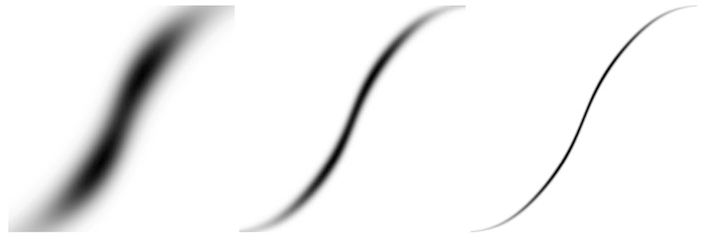
\includegraphics[width=.98\linewidth]{assets/ch06-fig-6-2.pdf}
\caption{一维传输问题中的最优$\gamma$（初始测度是中心高斯分布；到达测度由两个峰组成），由IPFP方法对逐渐减小的$\varepsilon$值计算得到. 右图相当精确地描述了最优的单调映射. 图片由L.~Nenna惠予提供.}\label{fig:6.2}
\end{figure}

这表明，$F$的极大化等价于$b_j=\int_{V_\psi(j)}f(x)\,\mathrm dx$，也使得可以用梯度方法寻找$F$的最大值. 为此，检验$F$的二阶导数的上界也很有用. 再把注意力限制在$c(x,y)=\frac12|x-y|^2$. 注意，将$\psi$的坐标值从$\psi_j$变到$\psi_j+h_j$，会使所有单元$V_\psi(j')$改变，但仅仅把常数$a(j,j')$改变$h_{j'}-h_j$的量. 这意味着定义其边界的超平面移动的距离为$\frac{|h|}{|y_{j'}-y_j|}$量级. 若点$y_j$固定且互异，则对称差$V_\psi(j')\mathbin{\Delta}W_{\psi+h}(j')$的测度有界于$C|h|$. 若$f\in L^\infty$，便得到
\begin{equation}\label{eq:6.4}
\left|\frac{\partial F}{\partial\psi_j}(\psi)
-\frac{\partial F}{\partial\psi_j}(\psi+h)\right|\le C|h|,
\end{equation}
以及$F\in C^{1,1}$.

\begin{sourcebox}{备忘：梯度算法}\label{box:6.8}\index{G071@梯度算法（gradient algorithm）|hyperpage}
若$F:\mathbb R^N\to\mathbb R$是可微凸函数，一个寻找$F$的最小值的简单算法是：取$x_0\in\mathbb R^N$及固定步长$\tau>0$，定义
\[
x_{k+1}=x_k-\tau\nabla F(x_k).
\]
若$F$满足对每个$x$都有$\alpha\mathrm I\le D^2F(x)\le L\mathrm I$，其中$\alpha,L>0$，则只要$\tau<2\alpha/L^2$，上述算法就以指数速度收敛. 更精确地，$F$严格凸且有唯一极小化元$\bar x$，并且$|x_k-\bar x|\le C\beta^k$，其中$\beta$依赖于$\tau,\alpha,L$，且在$\tau\in]0,2\alpha/L^2[$时$\beta<1$. $F(x_k)-\min F$的收敛同样为指数型.

若$D^2F$有上界但无下界（即$F$光滑但凸性不够强），而存在极小化元$\bar x$，则收敛速度要差得多：事实上，只能证明只要$\tau M<1$，就有$F(x_k)-F(\bar x)\le C/k$.

许多著作广泛介绍了凸优化中的梯度方法；更多细节可见例如\cite{b64}. 也有步长$\tau$随$k$变化的变体，变化方式既可以事先规定，也可以通过优化得到.

最后注意，上述算法也对应于离散化$F$的梯度流时的显式Euler格式（见备忘\autoref{box:8.1}）.
\end{sourcebox}

于是，这类梯度算法的实际实现，取决于怎样实际计算幂单元$V_\psi(j)$及其上的密度$f$的积分. 这属于所谓计算几何（computational geometry）的领域. 我们不对这一十分微妙的问题多作讨论，详细论述可见例如较近的论文\cite{b209,b233}. \cite{b233}提出了这些方法的原始实现，\cite{b209}又作了改进，并给出了几何形状之间最优传输的精彩数值模拟\footnote{下几页的图片由B.~Lévy惠予提供，采用与\cite{b209}相同的算法生成.}.

由于数值结果十分出色，我们通过\autoref{fig:6.3}和\autoref{fig:6.4}展示它们，也愿意对这一半离散设置中最高效的方法再多说一些.

事实上，\phantomsection\label{idx:i111-p244}\index{N111@Newton法（Newton’s method）|hyperpage}
尽管用梯度算法较容易描述，但改用Newton方法会收敛得快得多. Newton法（见\autoref{sec:6.3}中的\autoref{box:6.4}）适合寻找从$\mathbb R^N$到$\mathbb R^N$的向量函数的零点；这里的函数，将对偶势$\psi=(\psi_i)_i\in\mathbb R^N$映到各个值$b_i-\int_{V_\psi(i)}f(x)\,\mathrm dx=\partial F/\partial\psi_i$. 为能使用Newton法，需要能够计算这些值的导数，它们其实就是$F$的Hessian矩阵的元素. 还需证明该Hessian矩阵非奇异，并给出其特征值的下界. 这对应于$F$的一致凸性.

此外，已知Newton法只有在能够选择合适初始化时才高效，因为它只从某个邻域出发才收敛. \cite{b233}从多分辨率视角考虑问题，高效地处理了这一点. 给点族$y_j$配上若干个规模更小的点族，每个都由前一个通过Lloyd算法并按固定比例减少点数而得到. 这样，每个点族中的每个点，在下一个较小点族中都有唯一的像. 从最小点族的势$\psi$的计算开始，这很容易完成. 然后每步用第$i$个点族算出的势$\psi$，来构造下一步即第$(i-1)$个点族的Newton法初始化. 这保证了始终充分接近所寻找的极小化元，算法也能在极少次数的迭代中收敛. 实践中，\cite{b209}的实现能在几分钟内处理一百万个点.

\begin{figure}[htbp]
\centering
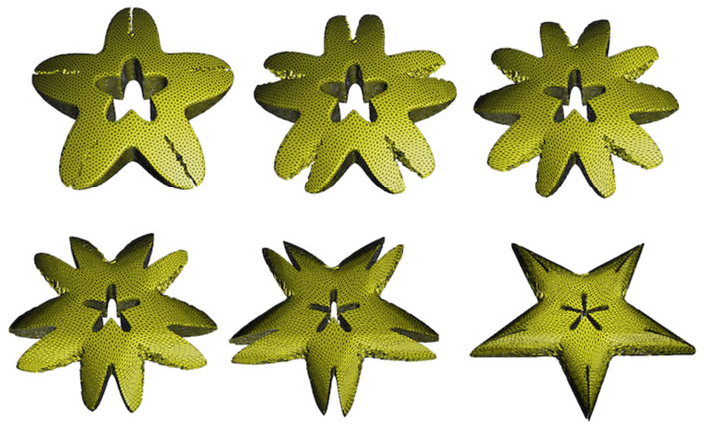
\includegraphics[width=.98\linewidth]{assets/ch06-fig-6-3.pdf}
\caption{三维中两颗不同星形之间的$W_2$测地线，利用单纯形剖分上的半离散最优传输计算得到. 获得剖分每个顶点$x_i$的像后，计算每个$x_i$与$\mathrm T(x_i)$之间的线性插值. 注意拓扑变化，以及星形每条分支上最优映射的奇性.}\label{fig:6.3}
\end{figure}

现在回到应用Newton过程所需的一致凸性的证明. 实际上，函数$F$远非严格凸：若给所有$\psi_i$加上同一常数，它就不变. 不过，除去这一不变性，可以期待它严格凸. 为此，需要固定某个值$\psi_{i_0}=0$，然后考察关于$i\ne i_0$的$\psi_i$的行为.

\begin{figure}[htbp]
\centering
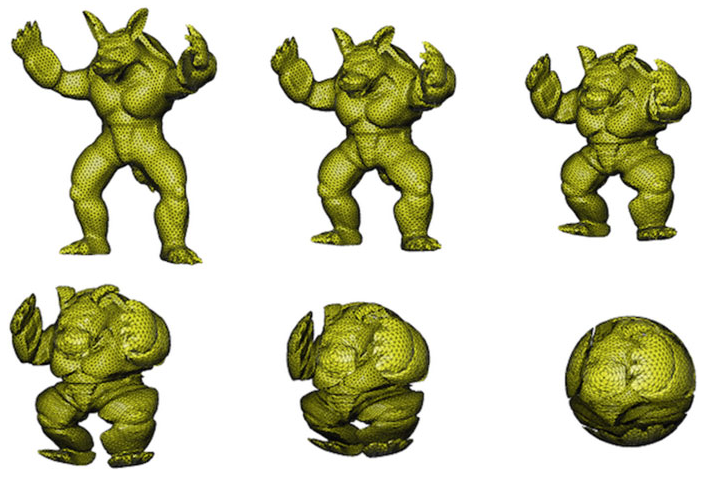
\includegraphics[width=.98\linewidth]{assets/ch06-fig-6-4.pdf}
\caption{“犰狳”形状上的均匀测度与球体上的均匀测度之间的$W_2$测地线（用至多一百万个Dirac质量离散）.}\label{fig:6.4}
\end{figure}

如何计算$F$的二阶导数？只需改进导出\eqref{eq:6.4}的计算：若$f$是连续密度，则得到
\[
\frac{\partial^2F}{\partial\psi_j\partial\psi_j}(\psi)
=-\frac1{|y_i-y_j|}\int_{\Gamma_{ij}}f(x)\,\mathrm d\mathscr H^{d-1}(x),
\qquad i\ne j,
\]
其中$\Gamma_{ij}=\partial V_\psi(i)\cap\partial V_\psi(j)$是对应于指标$i,j$的两个单元的公共边界（若存在），它是$(d-1)$维多面体. 对纯二阶导数，有
\[
\begin{aligned}
\frac{\partial^2F}{\partial^2\psi_i}(\psi)
&=\sum_{j\ne i}\frac1{|y_i-y_j|}
\int_{\Gamma_{ij}}f(x)\,\mathrm d\mathscr H^{d-1}(x)\\
&=-\sum_{j\ne i}\frac{\partial^2F}{\partial\psi_j\partial\psi_j}(\psi).
\end{aligned}
\]
注意，求和中也保留指标$i_0$. 这使我们能够写出一个关于$N$个变量的Hessian，它是奇异的，因为每一行的和为零. 然后去掉对应于$i_0$的行与列，就得到一个$(N-1)\times(N-1)$方阵$M$. 为检验$M$的可逆性，使用下面的引理：

\Needspace{10\baselineskip}
\begin{lemma}\label{obj:6.5}
任何满足以下性质的矩阵$M\in\mathrm M^{k\times k}$都可逆：
\begin{itemize}
\item[(H1)] 对所有$i$，$M^{i,i}\ge\sum_{j\ne i}|M^{i,j}|$；
\item[(H2)] 存在$i$使$M^{i,i}>\sum_{j\ne i}|M^{i,j}|$；
\item[(H3)] 对任意一对$(i,j)$，存在序列$i_1,i_2,\ldots,i_k$，其中$i_1=i$、$i_k=j$，满足$M^{i_h,i_{h+1}}\ne0$.
\end{itemize}
\end{lemma}
\begin{proof}
设$x\in\operatorname{Ker}(M)$，取使$|x_i|$最大的指标$i_0$. 为简便，可假设$x_{i_0}$为正. 则有
\[
\begin{aligned}
0&=M^{i_0,i_0}x_{i_0}-\sum_{j\ne i_0}M^{i_0,j}x_j\\
&\ge M^{i_0,i_0}x_{i_0}-\sum_{j\ne i_0}|M^{i_0,j}|x_{i_0}\\
&=x_{i_0}\left(M^{i_0,i_0}-\sum_{j\ne i_0}|M^{i_0,j}|\right)\ge0.
\end{aligned}
\]
这蕴含所有不等式都为等式，特别地，只要$M^{i_0,j}\ne0$，就有$x_j=x_{i_0}$. 因而，$x$在$i_0$所有“邻居”指标上的分量都等于$x_{i_0}$（并且也都是最大的）. 这使我们可以用另一个达到最大值的指标$j$替换$i_0$，重复论证，如此等等；由于每个指标都能通过一条邻居链与$i_0$相连，得到所有分量都相等. 但这意味着在核中选出的向量必为$(1,1,\ldots,1)$的倍数. 然而，由假设(H2)，并非所有行的元素之和都为零，因此这个向量不在核中. 这证明$M$可逆.
\end{proof}

在一些合理假设下，上面的引理可以用于$F$的Hessian（例如，应要求密度$f$的支集弧连通）.

这保证了$F$的Hessian在每一点都是严格正定矩阵（在固定$\psi_{i_0}=0$的势组成的空间$\mathbb R^{N-1}$上）. 为应用Newton法，还应从下方控制其特征值. 这一点更微妙，见\cite{b114}：文中既给出了上述引理的三个假设不足以得到这一界的反例，也给出了当矩阵$M$来自幂单元分割这一特殊情形的证明.

另外，既然说到了\cite{b114}中的论证，再强调一下同一论文描述的另一种半离散方法. \phantomsection\label{idx:i86-p247}\index{K086@Knothe映射（Knothe map）|hyperpage}
该方法的想法来自\autoref{sec:2.4}中关于Knothe传输的考虑. 事实上，我们证明了Knothe映射是对应于矩阵$\operatorname{diag}(1,\varepsilon,\varepsilon^2,\ldots,\varepsilon^{d-1})$的退化二次成本的最优传输映射的极限，因而可以从这样的映射（Knothe）出发，再让$\varepsilon$变化. Knothe映射容易计算，也能找到相应的单元\footnote{这就是源于上述想法、在\cite{b114}中实现的半离散方法. 还有一个连续对应物，即关于Kantorovich势$\psi_\varepsilon$的偏微分方程. \cite{b66}从理论角度研究了它，Bonnotte基于$\varepsilon=0$附近Nash--Moser隐函数定理的应用，证明了一个非平凡的适定性结果（一旦$\varepsilon>0$，方程就更正则）. 后来，同一作者也在\cite{b65}中开始实现这一方程的时间离散化. 注意，这个连续方法在某些方面既使人想起\autoref{sec:6.2}的AHT流（因为它从Knothe映射出发，时间连续但为数值计算而离散，并在演化中每个时刻都施加规定的像测度），又使人想起\autoref{sec:6.3}的LR Newton迭代（因为其基础偏微分方程基于Monge--Ampère方程的线性化）.}. 由于对Knothe映射而言最重要的是最后一个坐标，这些单元就是具有规定体积的水平条带. 注意，要使该方法可行，需要假设各点的$x_d$分量互异. 计算初始条件之后，运行一个$N-1$维常微分方程（$N$是到达测度的原子数），求出Kantorovich势$\psi(\varepsilon)$的演化. 为证明该常微分方程适定所需的计算，与上述计算类似，并能推知演化符合Lipschitz向量场的Cauchy问题的标准存在、唯一、稳定性与逼近理论. 因而，可以采用显式Euler格式的时间离散化来逼近解. 观察$\varepsilon$从$0$变到$1$时势$\psi_\varepsilon$的演化，还能计算相应的单元；它们从矩形条带变为凸多面体幂单元.

\autoref{fig:6.5}展示了以上述方法得到的一个简单单元序列.

\begin{figure}[htbp]
\centering
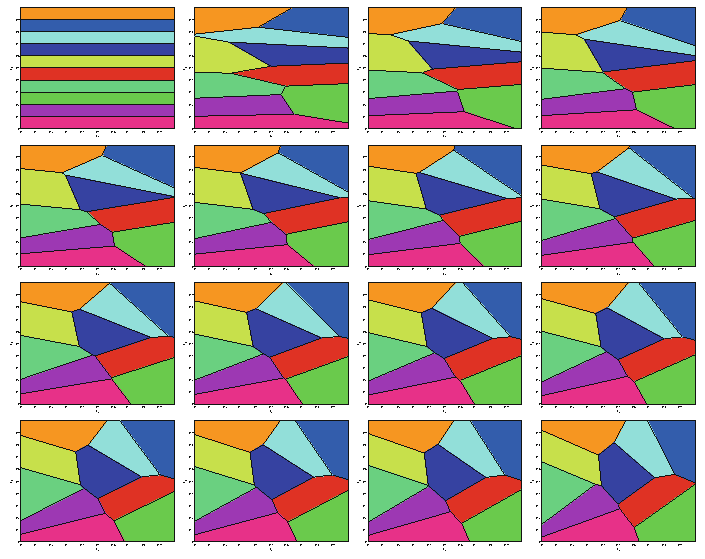
\includegraphics[width=.98\linewidth]{assets/ch06-fig-6-5.pdf}
\caption{十个样本点：$\varepsilon$从$0$到$1$时剖分的演化（从左上至右下）. 图片取自导向\cite{b114}的初步研究.}\label{fig:6.5}
\end{figure}
